\section{Open Linked data as a viable approach}

In the previous section, we identified some of the challenges smart cities will need to face in the following years. The data lifecycle model proposed at Figure \ref{fig:model} relies on Linked Open Data principles to try to solve these issues, reducing costs and enabling third parties to develop new business models on top of Linked Open Data.

Next we describe how Linked Open Data principles could help in the model's stages:

\subsection{Capture}

Data are the basis of smart cities, undoubtedly: services offered to citizens, decisions offered to city rulers by Decision Support Systems, all of them work thanks to big amounts of data. These data are captured from a wide variety of sources, like sensor networks installed along city, social networks or publicly available government data. In most cases, these sources publish data in a wide set of heterogeneous formats, forcing data consumers to develop different connectors for each source. As can be seen at section \ref{subsec:process}, there are a lot of different and widely extended ontologies which can represent data acquired from sources found in smart cities, easing the capture, integration and publication of data from heterogeneous domains. In this section, different sources of data which can be found in smart cities are shown, while in section \ref{subsec:process} the transformation process from their raw data to Linked Data is exposed. 

\subsubsection{Sensor Networks}\label{sensor_networks}

A sensor network is composed by low-cost, low-power, small sized and multifunctional sensor nodes which are densely deployed either inside the phenomenon or very close to it \cite{akyildiz_survey_2002}. In a smart city, these sensor networks are used for a wide range of applications, from the simple analysis of air quality\footnote{\url{http://helheim.deusto.es/bizkaisense/}} to the complex representation of public transport services\footnote{\url{http://traintimes.org.uk/map/tube/}}, through the sensors embedded in citizens smartphones. For example, the SmartSantander project envisions the deployment of 20,000 sensors in four European cities \cite{sanchez_smartsantander:_2011}. Nowadays due the existence of open-source and cheap hardware devices like Arduino\footnote{\url{http://www.arduino.cc/}} or Raspberry Pi\footnote{\url{http://www.raspberrypi.org/}}, the amount of collaborative and social sensor networks is growing faster and faster. Furthermore, there are software platforms like Xively\footnote{\url{https://xively.com}} or Linked Sensor Middleware \cite{le-phuoc_linked_2011}, which allow users to share the captured data from their own sensors networks in an easy way.

\subsubsection{Social Networks}\label{social_networks}

Since the adoption of the Web 2.0 paradigm \cite{oreilly_what_2007}, users have become more and more active when interacting with the Web. The clearest example of this transformation of the Web can be found in social networks and the high growth of their users. For example, at the end of the second quarter of 2013, Facebook has almost 1.2 billion users\footnote{\url{http://techcrunch.com/2013/07/24/facebook-growth-2/}}, while at the end of 2012, Twitter reached more than 200 million monthly active users\footnote{\url{https://twitter.com/twitter/status/281051652235087872}}. Although users of social networks generate a lot of data, it is hard to manipulate them because users write in a language not understood by machines. To solve this issue many authors have worked with different Natural Language Processing techniques. For example, NLP and Named Entity Recognition (NER) systems \cite{maynard_named_2001} can be used to detect tweets which talk about some emergency situation like a car crash, an earthquake and so on; and to recognize different properties about the emergency situation like the place or the magnitude of this situation \cite{sixto_enable_????,martins_machine_2010}. Extracting data from relevant tweets could help emergency teams when planning their response to different types of situations as can be seen at \cite{abel_twitcident:_2012,vieweg_microblogging_2010,hughes_twitter_2009}.


\subsubsection{Government Open Data}

Government Open Data has gained a lot of value in recent years, thanks to the proliferation of Open Data portals from different administrations of the entire World. In these portals, the governments publish relevant data for the citizens, in a heterogeneous set of formats like CSV, XML or RDF. Usually, data from these portals can be consumed by developers in an easy way thanks to the provided APIs, so there are a lot of applications developed over these data. As citizens are the most important part of smart cities, these applications make them an active part in the governance of the city.

To illustrate the importance of Government Open Data, in Table \ref{tab:open data portals} some Open Data portals are shown.

    \begin{table}
        \center
        \begin{tabular}{|p{2cm}|p{3cm}|p{2.5cm}|p{2cm}|}
            \hline
            \textbf{Name} & \textbf{Public Administration} & \textbf{No. of datasets (Sept. 2013)} & \textbf{API} \\
            \hline \hline
            Data.gov & Government of USA & 97,536 & REST, SOAP, WMS\\
            \hline
            Data.gov.uk & Government of UK & 10,114 & REST \\
            \hline
            Data.gc.ca & Government of Canada & 197,805 & REST \\
            \hline
            Open Data Euskadi & Government of Basque Country & 2,127 & RSS, Java API, REST \\
            \hline
            Datos Abiertos de Zaragoza & Council of Zaragoza & 112 & SPARQL \\
            \hline
        \end{tabular}
        \caption{Open Data portals around the World.}
        \label{tab:open data portals}
    \end{table}

As have been shown, in a smart city a lot of data sources can be found, publishing an abundant stream of interesting data in a different and heterogeneous manner. In section \ref{subsec:process}, how transform these data in a standard formats is shown.

\subsection{Process}
\label{subsec:process}

\subsection{Store}

\subsection{Publish}

\subsection{Discovery}
\label{subsec:discovery}

\subsection{Enrichment}

\subsection{Consume}

At this stage, the focus is located on consuming data for business-logic processes, should they involve data mining algorithms, analytics, reasoning, etc.

Whereas complex processing algorithms can be used independently of the dataset format, Linked Open Data can greatly help at reasoning purposes. Linked Open Data describes entities using ontologies, semantic constraints and restriction rules (belonging, domain, range, etc.) which favor the inference of new information from the existing one. Thanks to those semantics present in Linked Data, algorithms are not fed with raw values (numbers, strings...), but with semantically meaningful information (height in cm, world countries, company names...), thus resulting in higher quality outputs and making algorithms more error aware (i.e., if a given algorithm is in charge of mapping the layout of a mountainous region, and founds the height of one of the mountains to be \textit{3.45}, it is possible to detect the conversion has failed at some point, as height datatype was expected to be given in \textit{meters}).

As seen in sections \ref{sensor_networks} and \ref{social_networks}, sensors and social networks are common data input resources, generating huge amounts of data streamed in real time. The work done in \cite{sequeda2009linked} comprises a set of best practices to publish and link stream data to be part of the Semantic Web.

However, when it comes to consume Linked Data streams, SPARQL can find its limits \cite{della2009s}. Stream-querying languages such as CQELS's\footnote{\url{https://code.google.com/p/cqels/}} language (an extension of the declarative SPARQL 1.1 language using the EBNF notation) can greatly help in the task. CQELS\cite{le2011native} (Continuous Query Evaluation over Linked Stream) is a native and adaptive query processor for unified query processing over Linked Stream Data and Linked Data developed at DERI Galway\footnote{http://www.deri.ie/}.

Initially, a query pattern is added to represent window operators on RDF Stream:

\begin{lstlisting}
GraphPatternNotTriples ::= GroupOrUnionGraphPattern | 
OptionalGraphPattern | MinusGraphPattern | GraphGraphPattern | 
*StreamGraphPattern* | ServiceGraphPattern | Filter | Bind
\end{lstlisting}

Assuming that each stream has an IRI as identification, the \textit{StreamGraphPattern} is defined as follows:

\begin{lstlisting}
StreamGraphPattern ::= 'STREAM' '['Window']' VarOrIRIref '{'TriplesTemplate'}'
Window ::= Rangle|Triple|'NOW'|'ALL'
Range ::= 'RANGE' Duration ('SLIDE' Duration |'TUMBLING')?
Triple ::= 'TRIPLES' INTEGER
Duration ::= (INTEGER 'd'|'h'|'m'|'s'|'ms'|'ns')+
\end{lstlisting}

An example query could be:

\begin{lstlisting}
PREFIX lv: <http://deri.org/floorplan/>
PREFIX dc: <http://purl.org/dc/elements/1.1/> 
PREFIX foaf: <http://xmlns.com/foaf/0.1/> 
PREFIX xsd: <http://www.w3.org/2001/XMLSchema#>

SELECT ?locName FROM NAMED <http://deri.org/floorplan/> WHERE {
	STREAM <http://deri.org/streams/rfid> [NOW] 
	{?person lv:detectedAt ?loc} 
	{?person foaf:name "AUTHORNAME"^^xsd:string }
	
	GRAPH <http://deri.org/floorplan/> 
	{?loc lv:name ?locName}
}
\end{lstlisting}

Eventually, both batch and streamming results can be consumed through \textit{REST} services by web or mobile applications, or serve as input for more processing algorithms until they are finally presented to end-users.

\subsection{Visualize}

In order to make meaning from data, humans have developed a great ability to understand visual representations. The main objective of data visualization is to communicate information in a clean and effective way through graphical means. It's also suggested that visualization should also encourage users engagement and attention.

The \textit{"A picture is worth a thousand words"} saying reflects the power images and graphics have when expressing information, and can condense big datasets into a couple of representative, powerful images.

As Linked Data is based on subject-predicate-object triples, graphs are a natural way to represent triple stores, where subject and object nodes are inter-connected through predicate links. When further analysis is applied on triples, a diverse variety of representations can be chosen to show processed information: charts, infographics, flows, etc.\cite{khan2011data}

Browser-side visualization technologies such as d3.js\footnote{http://d3js.org/} (by Michael Bostock) and Raphaël\footnote{http://raphaeljs.com/} are JavaScript-based libraries to allow the visual representation of data on modern web browsers, allowing anybody with a minimum internet connection try to understand data patterns in a graphical form.

For developers not familiar with visualization techniques, some investigations are trying to enable the automatic generation of graphical representations of Linked Data query results. The \textit{LDVM} (Linked Data Visualization Model) \cite{brunetti2012linked} is proposed as a model to rapidly create visualizations of RDF data. \textit{LODVisualization}\footnote{http://lodvisualization.appspot.com/} is an implemented prototype which supports the LDVM.

Visualbox\footnote{http://alangrafu.github.io/visualbox/} is a simplified edition of LODSPeaKr\footnote{http://lodspeakr.org/} focused on allowing people create visualizations using Linked Data.

\begin{figure}
    \center
    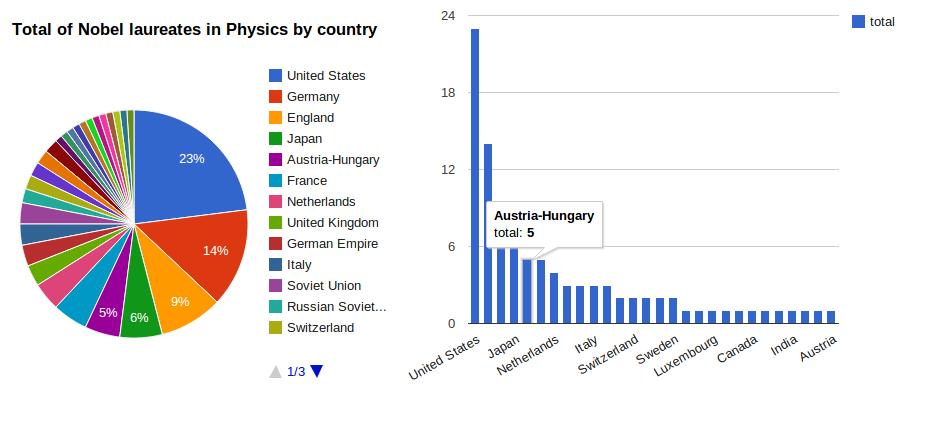
\includegraphics[width=\textwidth]{img/ld_approach/graph.png}
    \caption{Visualbox graph example (ownership: Alvaro Graves).}
\end{figure}

Independently of how visualizations are generated, they provide a perfect solution to present high-quality, refined data to end-users.